% This style is based on pandoc's default, but with lots of options removed.
\documentclass[letterpaper,table]{mysteries}
\usepackage{multicol}

% Set the typeface to use
\usepackage{fontspec}
\setmainfont{Crimson}

% No idea what these do yet
\usepackage{amssymb,amsmath}
\usepackage{fixltx2e} % provides \textsubscript

% Text Encoding
\usepackage[utf8]{inputenc}

% Enable upquote and microtype
\usepackage{upquote,microtype}
\UseMicrotypeSet[protrusion]{basicmath}

% Set page geometry
\usepackage[letterpaper, total={7in, 9.5in}, margin=1.5in]{geometry}

% This makes sure links are presented as just normal text
\usepackage{hyperref}
\hypersetup{unicode=true,
            pdfborder={0 0 0},
            breaklinks=true}
\urlstyle{same}  % don't use monospace font for urls

% Use xtab for tables
\usepackage{xtab}
\usepackage{booktabs}
\usepackage[table]{xcolor}
\definecolor{light-gray}{gray}{0.95}

% Use indexes!
\usepackage{imakeidx}
\makeindex

% Use csquotes for block quotes
\usepackage{csquotes}

% Image stuff
\usepackage{graphicx,grffile}
\usepackage[export]{adjustbox}
\graphicspath{ {./images/} } % sets the location for images
\makeatletter
\def\maxwidth{\ifdim\Gin@nat@width>\linewidth\linewidth\else\Gin@nat@width\fi}
\def\maxheight{\ifdim\Gin@nat@height>\textheight\textheight\else\Gin@nat@height\fi}
\makeatother
% Scale images if necessary, so that they will not overflow the page
% margins by default, and it is still possible to overwrite the defaults
% using explicit options in \includegraphics[width, height, ...]{}
\setkeys{Gin}{width=\maxwidth,height=\maxheight,keepaspectratio}

\usepackage{parskip}

\setlength{\emergencystretch}{3em}  % prevent overfull lines
\providecommand{\tightlist}{%
  \setlength{\itemsep}{0pt}\setlength{\parskip}{0pt}}

% Not sure what this does
\TeXXeTstate=1
\newcommand{\RL}[1]{\beginR #1\endR}
\newcommand{\LR}[1]{\beginL #1\endL}
\newenvironment{RTL}{\beginR}{\endR}
\newenvironment{LTR}{\beginL}{\endL}

% Begin the document
\begin{document}
\frontmatter
\thispagestyle{empty}

\begin{center}
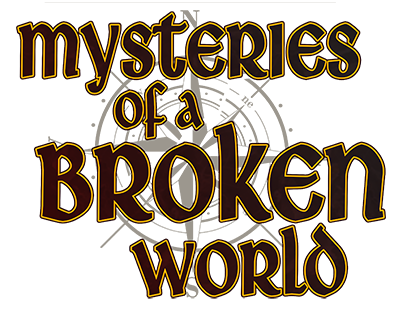
\includegraphics[center]{logo-mysteries}

By Ben Overmyer

Preview Copy

\today
\end{center}

\chapter{Credits}

\begin{multicols}{2}

\textbf{Author:} Ben Overmyer

\textbf{Editing:} Sarah Overmyer

\textbf{Playtesting:} Kevin Rohan

\textbf{Special Thanks To:} Salvorin

\end{multicols}


\setcounter{tocdepth}{2}
\tableofcontents
\newpage

\mainmatter
\chapter{Introduction}

\begin{multicols}{2}

An apocalypse destroyed the world as it used to be. No one knows what caused it or recalls what the old world was like. Most refer to the apocalypse as the Breaking of the World, or 'The Breaking' for short.

In the aftermath of the Breaking, most of the world has been overtaken with untamed wilderness. Scattered throughout the wilderness are the ruins of the old world, and occasionally a large town known as a freehold.

There is some trade between freeholds, but the distance and danger between them makes sharing supplies and knowledge difficult. Ruins are filled with artifacts and knowledge that could help your freehold survive and thrive. The wilds and the ruins also have an abundance of horrific, magic-twisted monsters.

You know little of the world outside of your freehold, but perhaps it’s time to start to learn more. It is up to you to help rebuild your community. Do you have the courage, skill, and luck to bring back treasures from the dark places? Will you save your Freehold from the encroaching wilds?

These are your stories now. Go forth, and uncover the Mysteries of a Broken World!

\end{multicols}

\chapter{Character Creation}

\begin{multicols}{2}

This chapter details the rules for creating the character you will play.
If your Mystery Weaver is providing characters for you, you can skip this
chapter.

\section{Summary of Character Creation}

\begin{enumerate}
	\item Roll ability scores
	\item Choose a bloodline
	\item Choose an archetype
	\item Choose a background
	\item Choose an alignment
	\item Roll for afflictions
	\item Choose spells, if applicable
	\item Roll for mana points, if applicable
	\item Roll for hit points
	\item Roll for starting money
	\item Fill out details, as desired
\end{enumerate}

\section{Ability Scores}

For each of the six scores, roll 3d6.

You may swap two scores once after you've finished rolling, OR you can reroll
all six scores once.

\textbf{Strength:} A measure of your physical might. Governs how much damage you
do in melee combat.

\textbf{Dexterity:} Your agility and deftness. Affects your ranged combat damage
and when you act in combat.

\textbf{Constitution:} A reflection of your physical and mental endurance. This
affects your total Hit Points as well as your resistances.

\textbf{Wisdom:} This is a measure of your common sense and understanding of the
ways of the world. It is vital for adherents of the divine.

\textbf{Intelligence:} This is how clever and learned you are. It affects arcane
spellcasting and how many languages you know.

\textbf{Charisma:} This is your social ability, force of personality, and general
attractiveness. It affects how many NPC retainers you can have, as well as
leadership and persuasion.

\section{Bloodline}

Choose one of the following as your bloodline. The bloodlines found in any given Freehold
vary greatly.

\subsection{Dwarf}

\textbf{Adulthood:} 50 years

\textbf{Maximum Age:} 300 years

Dwarves are short and stocky. Both men and women can grow prodigious beards.
They have a natural affinity for stone and can navigate underground as if they
could see for miles.

\subsection{Elf}

\textbf{Adulthood:} 50 years

\textbf{Maximum Age:} Unknown

Elves are thin, tall, and elegant. Their ears are pointed. They live eternally
unless slain. Elves are agile and quick and have an affinity for magic. No living
elf is old enough to remember the Breaking.

\subsection{Halfling}

\textbf{Adulthood:} 20 years

\textbf{Maximum Age:} 200 years

Halflings are short, but normally proportioned for their size. They have
large, hairy feet and usually go barefoot. Many seem to have a knack for
moving quietly.

\subsection{Human}

\textbf{Adulthood:} 18 years

\textbf{Maximum Age:} 100 years

Humans vary greatly in appearance and demeanor. Their skin ranges in color
from deepest black to palest white, with no one hue being more common than
the others.

\subsection{Minotaur}

\textbf{Adulthood:} 20 years

\textbf{Maximum Age:} 150 years

Minotaurs are large, bulky humanoids with the head and horns of a bull. They
tower over most other bloodlines.

\subsection{Sandman}

\textbf{Adulthood:} 20 years

\textbf{Maximum Age:} 100 years

Sandmen are humanoids that appear to be made of sand. Their eyes are glassy and
their skin is yellow or brown. They feel no heat or cold.

\section{Archetype}

Choose one of the following. This is your character's primary profession and
the source of your main abilities. It also gives you your Hit Die.

\subsection{Alchemist}

\textbf{Hit Die:} d4

\textbf{Armor Allowed:} Leather, Padded

\textbf{Weapons Allowed:} Any one-handed

Alchemists are brewers of potions and transmuters of materials. They have a
greater understanding of the laws of the natural world than most others. An
alchemist may craft potions.

\subsection{Berserker}

\textbf{Hit Die:} d10

\textbf{Armor Allowed:} None

\textbf{Weapons Allowed:} Any

Berserkers are warriors who have made a pact with the spirit of Fury. During
battle they may give themselves over to Fury, gaining great strength and speed.
However, they have no control over their actions until Fury releases them.

\subsection{Bard}

\textbf{Hit Die:} d4

\textbf{Mana Die:} d6

\textbf{Armor Allowed:} Leather, Padded

\textbf{Weapons Allowed:} Any one-handed

Bards are musicians who weave magic into their songs. They might use musical
instruments or rely only on their voice. Their magic is subtle and moving.
Bards may learn spells from the Enchantment list.

\subsection{Demon-Caller}

\textbf{Hit Die:} d4

\textbf{Mana Die:} d8

\textbf{Armor Allowed:} None

\textbf{Weapons Allowed:} One-handed melee

Demon-callers are aggressive magic-users who derive their power from dark entities.
They have made pacts to gain power, and must serve the ends of their patron.
A demon-caller may learn spells from the Demonic list.

\subsection{Man-At-Arms}

\textbf{Hit Die:} d6

\textbf{Armor Allowed:} Any

\textbf{Weapons Allowed:} Any

Men-at-arms are professional soldiers. Their craft is war. They are proficient
in the use of all weapons and armor. A man-at-arms may choose one weapon to
specialize in, and from that point forward, gain a +1 to hit with that weapon.

\subsection{Monk}

\textbf{Hit Die:} d8

\textbf{Armor Allowed:} Padded

\textbf{Weapons Allowed:} None

Monks are warriors of a particular church. They eschew the use of weapons and
armor in favor of perfecting unarmed combat. Each church has a different style
of fighting, usually themed after the tenets of their patron god.

\subsection{Paladin}

\textbf{Hit Die:} d8

\textbf{Armor Allowed:} Any

\textbf{Weapons Allowed:} Any

Paladins are zealous soldiers of a particular church. They adhere strictly to
a code of conduct, even when that adherence puts them or others at risk. A
paladin may heal another fully by touching them and invoking their deity once per day.

\subsection{Priest}

\textbf{Hit Die:} d6

\textbf{Mana Die:} d6

\textbf{Armor Allowed:} Leather, Padded, Chain

\textbf{Weapons Allowed:} Any blunt

Priests are the voices of the gods. They adhere rigidly to the rituals and
practices of their church, and in exchange, are given the ability to work
miracles. Priests may use spells from the Divine list. They may also Turn
Undead.

\subsection{Ranger}

\textbf{Hit Die:} d6

\textbf{Armor Allowed:} Leather, Padded

\textbf{Weapons Allowed:} Any ranged, one-handed melee

Rangers are woodland archers and hunters. Their proficiency in stealth is
unmatched. They know the woods more than any other mortal. A ranger gains +1 to
hit with bows.

\subsection{Channeler}

\textbf{Hit Die:} d4

\textbf{Mana Die:} d12

\textbf{Armor Allowed:} None

\textbf{Weapons Allowed:} One-handed melee

Channelers are arcane spellcasters that do not rely on book learning for their
magic. Instead, they may innately cast spells. Channelers only get spells from
the Elemental list. They may not learn spells from any external source. Instead,
every time a channeler gains a level, he chooses one new spell from the Elemental
list.

\subsection{Thief}

\textbf{Hit Die:} d6

\textbf{Armor Allowed:} Leather, Padded

\textbf{Weapons Allowed:} Any one-handed

Thieves are rogues and highwaymen. They are skilled at sneaking into places and
stealing whatever valuables may lie therein. A thief excels at picking locks,
disarming or setting traps, and is a master of all forms of stealth.

\subsection{Tree-Speaker}

\textbf{Hit Die:} d4

\textbf{Mana Die:} d8

\textbf{Armor Allowed:} Leather, Padded

\textbf{Weapons Allowed:} Any one-handed

Tree-speakers are spellcasters in tune with the natural world. They revere nature
and work to protect it and maintain its balance. Tree-speakers may use spells from
the Nature list.

\subsection{Wizard}

\textbf{Hit Die:} d4

\textbf{Mana Die:} d8

\textbf{Armor Allowed:} None

\textbf{Weapons Allowed:} One-handed melee

Wizards are arcane scholars and practitioners of High Magic. They study the inner
workings of magic and seek to unlock its deepest secrets. Wizards may learn
spells from any list other than Divine or Demonic.

\section{Background}

The following reflects a profession or calling that your character had prior
to picking up the mantle of adventurer, or that their parents wanted them to
pick up, or something along those lines. It represents your general area of
knowledge, as well as some specific skills you might apply when not off
adventuring.

You may choose one, or roll 1d100 on the table.

\bottomcaption{List of backgrounds}
\tablefirsthead{\hline \multicolumn{1}{|c|}{\textbf{Roll}} &
											 \multicolumn{1}{c|}{\textbf{Background}} \\ \hline }
\begin{center}
{\rowcolors{3}{white}{light-gray}
\begin{xtabular}{|l|l|}
01-02 & Apothecary \\
03-04 & Armorer \\
05-06 & Astronomer \\
07-08 & Baker \\
09-10 & Barber \\
11-12 & Barrister \\
13-14 & Blacksmith \\
15-16 & Bookbinder \\
17-18 & Bowyer \\
19-20 & Brewer \\
21-22 & Bricklayer \\
23-24 & Butler \\
25-26 & Candlemaker \\
27-28 & Carpenter \\
29-30 & Cartographer \\
31-32 & Chaplain \\
33-34 & Cook \\
35-36 & Courtesan \\
37-38 & Dyer \\
39-40 & Engraver \\
41-42 & Falconer \\
43-44 & Farmer \\
45-46 & Fisherman \\
47-48 & Fortune Teller \\
49-50 & Furrier \\
51-52 & Gardener \\
53-54 & Glassblower \\
55-56 & Gravedigger \\
57-58 & Herald \\
59-60 & Horse Trainer \\
61-62 & Hunter \\
63-64 & Innkeeper \\
65-66 & Jester \\
67-68 & Leatherworker \\
69-70 & Merchant \\
71-72 & Moneylender \\
73-74 & Musician \\
75-76 & Painter \\
77-78 & Poet \\
79-80 & Potter \\
81-82 & Rat Catcher \\
83-84 & Sailor \\
85-86 & Scout \\
87-88 & Scribe \\
89-90 & Sculptor \\
91-92 & Shipwright \\
93-94 & Shoemaker \\
95-96 & Squire \\
97-98 & Town Guard \\
99-00 & Trapper \\
\hline
\end{xtabular}
}
\end{center}

\section{Alignment}

Your character's alignment reflects what primal force influences their life.
It may manifest subtly, such as in influencing your character's decisions.
It may also manifest dramatically, such as a monster with the same alignment
appearing in the area. Such major manifestations are rare, however.

Characters can only use magical items that share their own alignment, or have
no alignment.

\textbf{Equilibrium:} The primal force of Equilibrium seeks to limit all other
forces. Those who align with Equilibrium are just, merciful, or callous.

\textbf{Chaos:} The primal force of Chaos seeks continual renewal and change. Those
who align with Chaos are impulsive, brash, or mercurial.

\textbf{Destiny:} The primal force of Destiny seeks continuity and predictability.
Those who align with Destiny are imperious, fatalistic, or resilient.

\textbf{Void:} The primal force of Void seeks emptiness, clarity, and purity. Those
who align with Void are thoughtful, stern, or aloof.

\section{Afflictions}

Afflictions are random mutations caused either by mutant parentage or by
encountering a place of wild magic left over from the Breaking. Regardless
of whether the Affliction has a positive effect or not, all those who have
an Affliction are shunned by normal society. They are regarded as the
Afflicted.

Your character has a chance to have an Affliction at character creation. Roll
1d100. If the result is 3 or less, roll 1d100 on the following table.

\bottomcaption{List of afflictions}
\tablefirsthead{\hline \multicolumn{1}{|c|}{\textbf{Roll}} &
											 \multicolumn{1}{c|}{\textbf{Affliction}} \\ \hline }
\begin{center}
{\rowcolors{3}{white}{light-gray}
\begin{xtabular}{|l|l|}
01-03 & Albinism \\
04-08 & Allergies \\
09-10 & Black and White Vision \\
11-13 & Claws \\
14-19 & Color Blindness \\
20-21 & Dwarfism \\
22-25 & Enhanced Sense of Smell \\
26-28 & Extra Fingers \\
29-33 & Fangs \\
34-35 & Forked Tongue \\
36-39 & Functional Gills \\
40-41 & Fur \\
42-46 & Gigantism \\
47-50 & Hairless \\
51-53 & Horns \\
54-55 & Occasional Seizures \\
56-60 & Odd Hair Color \\
61-67 & Oddly Colored Skin \\
68-69 & Permanent Boils \\
70-73 & Scaly Skin \\
74-75 & Strong Body Odor \\
76-78 & Tail \\
79-81 & Third Eye \\
82-84 & Thorny Skin \\
85-96 & Unnatural Eyes \\
97-98 & Webbed Feet \\
99-99 & Weird Voice \\
00-00 & Roll Again Twice \\
\hline
\end{xtabular}
}
\end{center}

\section{Spells}

If your character has a spellcasting archetype, then choose one spell from the
appropriate spell lists. This is the spell that your character knows at
the start of their journey.

\section{Mana Points}

If your character has a spellcasting archetype, then roll the Mana Die of your
archetype. If the result is a 1, you may reroll once. If your Intelligence
is higher than 12, add 1 to the result. This is your maximum Mana Points.

\section{Hit Points}

Look up the Hit Die of your archetype. Roll one of those dice. If the result is a
1 or a 2, you may reroll once. If your Constitution is higher than 12, add 1
to the result. This is your maximum Hit Points.

\section{Starting Money}

Your character begins the game with 3d6 x 10 silver coins. You can use this
money to buy starting equipment. See the Equipment chapter for a list of
things that you can buy. Adventurers typically are given this money by the
freehold they belong to, but the money may come from other sources.

\section{Character Details}

You may wish to write down a few extra details about your character, though
this is not required. Some things you might want to think about are:

\begin{itemize}
	\item Age
	\item Gender
	\item Weight
	\item Height
	\item Hair Color and Style
	\item Eye Color
	\item Skin Color
	\item Body Shape
	\item Family
	\item Hobbies
	\item Motivations
	\item Core Beliefs
\end{itemize}

\section{Advancement}

Your character will gain Experience Points for bringing treasure and knowledge
back from the wilds. Experience Points (or XP for short) are only gained once
your character returns what they've found to the rulership of their Freehold.

Once you have earned enough XP, you will gain a level. Once you do so, you roll
your archetype Hit Die and add the result to your maximum Hit Points. If your
Constitution score is higher than a 12, you add 1 to this total each time you
level up.

If you have a spellcasting archetype, the maximum level of spell that you can cast
increases by 1 each time you level up. So, if you are level 3, you can cast up
to (and including) level 3 spells. Also, roll your archetype Mana Die and add the
result to your maximum Mana Points. If your Intelligence score is higher than a
12, you add 1 to this total each time you level up.

Levels are gained every 1,000 XP.

\section{Learning Spells}

New spells are only gained by learning them from artifacts found in the ruins
of the old world. Most often, these will be spell scrolls or books. Another
spellcaster who knows the spell you seek to learn may be able to teach it to
you, but you must meet the level and spell list restrictions in order to
learn it.

Learning a new spell takes a number of weeks equal to the spell's level. The
caster must spend that time studying and practicing.

\end{multicols}

\chapter{Equipment}

\begin{multicols}{2}

The following is a list of all the equipment that
characters might buy or otherwise acquire through
their adventures.

Note: because freeholds are isolated and have little
in the way of resources, it's unlikely that any given
freehold will have everything in these lists.

In particular, things that require a lot of artisanal
skill to create—like full plate—are going to be
extremely rare.

\section{Costs and Currency}

After the breaking of the world, there was no central
authority to control the value of coinage. As such, no
one currency is considered to be the standard.

Much coinage still exists in the world, but it's judged
by its weight and not its appearance.

For simplicity's sake, all costs in this chapter are
given in gold coins (gc), silver coins (sc), copper
coins (cc), or pieces of eight (pe).

A gold coin is worth ten silver coins.

A silver coin is worth ten copper coins.

So, a gold coin is worth a hundred copper coins.

Also, copper coins are often cut into pieces for smaller
transactions. A single coin will be cut into eight pieces,
and so "pieces of eight" are used for things that cost
less than a copper coin.

Most people do not have a steady income. However, the
average village craftsman will likely earn roughly
8 gc over the course of a year in a freehold.

\end{multicols}

\section{Armor}

\bottomcaption{Types of armor}
\tablefirsthead{\hline \multicolumn{1}{|c|}{\textbf{Type}} &
											 \multicolumn{1}{c|}{\textbf{Armor Class}} &
											 \multicolumn{1}{c|}{\textbf{Cost}} \\ \hline }
\begin{center}
{\rowcolors{3}{white}{light-gray}
\begin{xtabular}{|l|l|l|}
Padded & 11 & 2 gc \\
Leather & 12 & 5 gc \\
Chain & 13 & 12 gc \\
Splint & 14 & 17 gc \\
Scale & 15 & 24 gc \\
Breastplate & 16 & 50 gc \\
Full Plate & 17 & 150 gc \\
\hline
\end{xtabular}
}
\end{center}

\section{Shields}

Shields increase the user's Armor Class by 1 if worn.
Note: tower shields are not meant to be worn, but rather
to be used as mobile walls.

\bottomcaption{Types of shields}
\tablefirsthead{\hline \multicolumn{1}{|c|}{\textbf{Type}} &
											 \multicolumn{1}{c|}{\textbf{Cost}} \\ \hline }
\begin{center}
{\rowcolors{3}{white}{light-gray}
\begin{xtabular}{|l|l|}
Buckler & 2 gc \\
Heater & 4 gc \\
Tower & 20 gc \\
\hline
\end{xtabular}
}
\end{center}

\section{Weapons}

\bottomcaption{List of afflictions}
\tablefirsthead{\hline \multicolumn{1}{|c|}{\textbf{Weapon}} &
											 \multicolumn{1}{c|}{\textbf{Hands}} &
											 \multicolumn{1}{c|}{\textbf{Type}} &
											 \multicolumn{1}{c|}{\textbf{Melee/Ranged}} &
											 \multicolumn{1}{c|}{\textbf{Cost}} \\ \hline }
\begin{center}
{\rowcolors{3}{white}{light-gray}
\begin{xtabular}{|l|l|l|l|l|}
Two-handed Axe & 2 H & Slashing Melee & 7 gc \\
Hand axe & 1 H & Slashing Melee & 4 gc \\
Short Sword & 1 H & Slashing Melee & 7 gc \\
Longsword & 1 H & Slashing Melee & 10 gc \\
Two-handed Sword 2 H & Slashing Melee & 15 gc \\
Staff & 2 H & Blunt & Melee & 5 sc \\
Dagger & 1 H & Piercing Melee & 1 sc \\
Pick & 1 H & Piercing Melee & 1 gc \\
Morningstar & 1 H & Blunt & Melee & 5 gc \\
Mace & 1 H & Blunt & Melee & 3 gc \\
Maul & 2 H & Blunt & Melee & 6 gc \\
Warhammer & 1 H & Blunt & Melee & 5 gc \\
Trident & 2 H & Piercing Melee & 5 gc \\
Spear & 2 H & Piercing Melee & 2 gc \\
Polearm & 1 H & Piercing Melee & 7 gc \\
Flail & 1 H & Blunt & Melee & 4 gc \\
Whip & 1 H & Blunt & Melee & 6 sc \\
Sling & 1 H & Blunt & Ranged & 5 cc \\
Shortbow & 2 H & N/A & Ranged & 3 gc \\
Longbow & 2 H & N/A & Ranged & 8 gc \\
Crossbow & 2 H & N/A & Ranged & 10 gc \\
Arrows x10 & N/A & Piercing N/A & 5 sc \\
Crossbow Bolts x5 N/A & Piercing N/A & 1 gc \\
\hline
\end{xtabular}
}
\end{center}

\textbf{Note:} You can use bows as a blunt weapon, but they will break
the first time you do this. After that, they are useless until
repaired.

\section{Tools}

These tools are readily available in most freeholds.

\bottomcaption{Types of tools}
\tablefirsthead{\hline \multicolumn{1}{|c|}{\textbf{Type}} &
											 \multicolumn{1}{c|}{\textbf{Cost}} \\ \hline }
\begin{center}
{\rowcolors{3}{white}{light-gray}
\begin{xtabular}{|l|l|}
Anvil & 1 gc \\
Armorer's tools & 13 gc \\
Augur & 2 pe \\
Backpack 5 sc \\
Bellows & 1 gc \\
Hammer & 1 cc \\
Hand mirror & 1 gc \\
Iron spike & 1 pe \\
Rope (50ft) & 1 cc \\
Sack, large & 5 cc \\
Sack, small & 1 cc \\
Shovel & 2 pe \\
Spade & 1 pe \\
Torch & 1 cc \\
Vise & 6 sc \\
\hline
\end{xtabular}
}
\end{center}

\section{Food and Drink}

Most common items found in inns and country houses are
listed here. More exotic foods and drinks are covered
in the world-building chapter.

\bottomcaption{Types of food and drink}
\tablefirsthead{\hline \multicolumn{1}{|c|}{\textbf{Type}} &
											 \multicolumn{1}{c|}{\textbf{Cost}} \\ \hline }
\begin{center}
{\rowcolors{3}{white}{light-gray}
\begin{xtabular}{|l|l|}
Ale (good), 1 barrel & 4 sc \\
Ale (good), 1 mug & 2 pe \\
Ale (poor), 1 barrel & 2 sc \\
Ale (poor), 1 mug & 1 pe \\
Egg & 1 pe \\
Fish (fried) & 2 pe \\
Fish (salted) & 4 pe \\
Handful of sugar & 1 sc \\
Haunch of meat & 1 cc \\
Loaf of bread & 1 pe \\
Meat stew & 5 pe \\
Side of Bacon & 6 cc \\
Wedge of cheese & 1 pe \\
Wine (good), 1 bottle & 9 pe \\
Wine (poor), 1 bottle & 3 pe \\
\hline
\end{xtabular}
}
\end{center}

\section{Livestock}

While adventuring or traveling for long periods of time,
it may be helpful to have a ready meat source available.

\bottomcaption{Types of livestock}
\tablefirsthead{\hline \multicolumn{1}{|c|}{\textbf{Type}} &
											 \multicolumn{1}{c|}{\textbf{Cost}} \\ \hline }
\begin{center}
{\rowcolors{3}{white}{light-gray}
\begin{xtabular}{|l|l|}
Chicken & 4 pe \\
Cow & 4 sc \\
Goat & 1 sc \\
Goose & 6 pe \\
Sheep & 2 sc \\
\hline
\end{xtabular}
}
\end{center}

\section{Horses}

Horses are valuable. A single quarterhorse is likely the most
expensive thing a typical farmer owns. In the world after the
Breaking, horses that are formally trained for battle are
almost unheard of.

\bottomcaption{Types of horses}
\tablefirsthead{\hline \multicolumn{1}{|c|}{\textbf{Type}} &
											 \multicolumn{1}{c|}{\textbf{Cost}} \\ \hline }
\begin{center}
{\rowcolors{3}{white}{light-gray}
\begin{xtabular}{|l|l|}
Quarterhorse & 1 gc \\
Riding horse & 10 gc \\
Warhorse & 1,000 gc \\
\hline
\end{xtabular}
}
\end{center}

\section{Housing}

Building a house requires land ownership or rent, if you're
building it near a freehold. If you're building in the wilderness,
good luck to you.

Renting a room for a night at an inn varies, but is commonly
less than a copper coin.

\bottomcaption{Types of housing}
\tablefirsthead{\hline \multicolumn{1}{|c|}{\textbf{Type}} &
											 \multicolumn{1}{c|}{\textbf{Cost}} \\ \hline }
\begin{center}
{\rowcolors{3}{white}{light-gray}
\begin{xtabular}{|l|l|}
Cottage & 10 gc \\
Craftman's house & 40 gc \\
Merchant's house & 120 gc \\
Noble's house & 500 gc \\
\hline
\end{xtabular}
}
\end{center}

\chapter{Spells}

\begin{multicols}{2}

This chapter lists all of the spells available to characters.

\section{Demonic, Level One}

\subsection{Beetle Boils}

\textbf{Range:} 25'

\textbf{Duration:} 2 rounds

\textbf{Mana Point Cost:} 2

You hurl a bag of dried beetle wings and cow's blood at the
victim. Their body is immediately covered, head to toe, in
painful boils. At the end of the spell, the boils burst and
small beetles erupt forth from them. The burst causes 1d4
damage and horrifies the victim. The beetles will fly away
from the victim. These beetles have the essence of their
victim within them, and may be used as components for spells
that require such.

\subsection{Ferocious Corruption}

\textbf{Range:} Infinite

\textbf{Duration:} 24 hours

\textbf{Mana Point Cost:} 3

You create an effigy of a specific living thing. The effigy must
be made with some part of the thing in question, whether a hair
or blood or other piece. As soon as you submerge the effigy in
a concoction of wine and blood, the victim becomes angrier
and more aggressive, even towards friends.

\subsection{Withering Touch}

\textbf{Range:} Touch

\textbf{Duration:} Instantaneous

\textbf{Mana Point Cost:} 2

You touch a living thing and drain its life essence, causing 1d8
damage and making the target visibly weaker and shrivelled. In
humanoids, this can take the form of an almost skeletal appearance,
with sunken eyes and skin stretched thinly over the bones. The
appearance effect lasts until the victim gets a good night's sleep.

\section{Demonic, Level Two}

\subsection{Curse of Eyes}

\textbf{Range:} 25'

\textbf{Duration:} 1 day

\textbf{Mana Point Cost:} 2

You gaze at a creature within range and your eyes flash red for a
moment. For the duration of the spell, the affected creature feels
a strong sense that they are being watched. Additionally, you can
occasionally sense what the victim is feeling, no matter how far
away you are. This only extends to emotions and not to physical
senses or thoughts.

\subsection{Plague of Bones}

\textbf{Range:} Touch

\textbf{Duration:} 1d4 rounds

\textbf{Mana Point Cost:} 2

You stab a creature with a bone shard inscribed with unholy symbols.
For the duration of the spell, they are wracked by sharp pain as
their bones grow millions of tiny spines. This deals 2d6 damage.
After the spell ends, the spines vanish, but the creature's bones
will always bear the same symbols that you inscribed on the shard.

\section{Divine, Level One}

\subsection{Censure}

\textbf{Range:} 25'

\textbf{Duration:} 1 round

\textbf{Mana Point Cost:} 1

You cry out a brief declaration at the victim, and they are
immediately brought to their knees. They are forced to remain
that way for the duration of the spell.

\subsection{Consecrate Ground}

\textbf{Range:} Special

\textbf{Duration:} 24 hours

\textbf{Mana Point Cost:} 3

By tracing the intended area of effect with your footsteps while
chanting a prayer to your patron deity, you consecrate the area
in their name. For the duration of the spell, any creatures opposed
to the will of your patron deity find it difficult to enter the
affected area. Entering the area causes them physical pain,
though it does no damage. You may trace an area of any size or
shape, as long as you are able to complete the tracing of the area
within a single recitation of your prayer. The area extends up to
ten feet above and below the area traced.

\subsection{Ease Pain}

\textbf{Range:} Touch

\textbf{Duration:} Instantaneous

\textbf{Mana Point Cost:} 2

You lay a hand on a creature or person and they immediately feel
better, both physically and mentally. They regain 1d4+1 lost Hit
Points and any suffering they are undergoing is reduced in
severity.

\section{Elemental, Level One}

\subsection{Dampen}

\textbf{Range:} Touch

\textbf{Duration:} Instantaneous

\textbf{Mana Point Cost:} 1

The object or living thing that you touch becomes covered in a fine
mist of water. It's not enough to douse a flame, but it may deter
a flame from starting.

\subsection{Fresh Air}

\textbf{Range:} 50'

\textbf{Duration:} Instantaneous

\textbf{Mana Point Cost:} 1

You clap your hands together and all of the air in range of the spell
is immediately clean and clear. If there's a vacuum, it is filled
with clean air. Anyone in range of the spell that is asphyxiating
can immediately breathe again, if only for a moment.

\subsection{Kindle Flame}

\textbf{Range:} 5'

\textbf{Duration:} Instantaneous

\textbf{Mana Point Cost:} 1

A nonliving, flammable object within range suddenly lights on fire.
The initial flame is no bigger than the palm of a hand, but it can
spread quickly.

\subsection{Minor Quake}

\textbf{Range:} 20'

\textbf{Duration:} 1 round

\textbf{Mana Point Cost:} 2

For the duration of the spell, a 3' radius circle of earth within
range shakes and rumbles. Any creatures standing on the affected
area are thrown off balance. Any actions they attempt that require
a dice roll have a -1 penalty.

\section{Elemental, Level Two}

\subsection{Find Water}

\textbf{Range:} 1 mile

\textbf{Duration:} 10 minutes

\textbf{Mana Point Cost:} 2

Any sources of water within range become known to the
caster. Whether they are salt water or fresh, drinkable
or not, also becomes known. For the duration of the
spell, the caster is aware of exactly how far away and
in what direction each source of water is.

\section{Enchantment, Level One}

\subsection{Charm Small Animals}

\textbf{Range:} 10'

\textbf{Duration:} 1 hour

\textbf{Mana Point Cost:} 1

All non-magical animals in range of the spell that are smaller than
a dog are immediately friendly towards you. They enjoy your company
and will protect you from threats as long as their own safety is
not threatened.

\subsection{Levity}

\textbf{Range:} 30'

\textbf{Duration:} 5 minutes

\textbf{Mana Point Cost:} 2

A creature in range is suddenly possessed of great joy and happiness.
It is far less likely to be hostile, and far more likely to be
friendly. The effect is cancelled if the creature is attacked or
otherwise harmed.

\subsection{Lighten}

\textbf{Range:} Touch

\textbf{Duration:} 24 hours

\textbf{Mana Point Cost:} 2

For the duration of the spell, the object or living thing that you touch
weighs half as much as it normally does.

\subsection{Obscure Object}

\textbf{Range:} Touch

\textbf{Duration:} 10 minutes

\textbf{Mana Point Cost:} 2

An object smaller than a housecat becomes difficult to
see for the duration of the spell. It doesn't become
invisible; rather, anyone looking in its direction finds
their attention shifts away from it and they can't quite
make out what it is. Only the caster is able to see the
object normally.

\section{Gate Magic, Level One}

\subsection{Blink Object}

\textbf{Range:} 10'

\textbf{Duration:} Instantaneous

\textbf{Mana Point Cost:} 1

A nonliving object smaller than a door is instantly teleported
up to five feet away from its original position. It must teleport
to an empty space, and it doesn't necessarily teleport exactly
to the point specified.

\subsection{Message}

\textbf{Range:} 10 miles

\textbf{Duration:} Instantaneous

\textbf{Mana Point Cost:} 2

You write a letter in magical characters on a simple piece of
paper. After you chant a few brief words and touch the letter,
it immediately vanishes. The recipient of the letter sees the
words of the letter appear in the air before them in a language
they can read. As soon as they finish reading the letter, or
if ten minutes pass, the words vanish.

\subsection{Second Step}

\textbf{Range:} Touch

\textbf{Duration:} 10 minutes

\textbf{Mana Point Cost:} 2

For the duration of the spell, the creature that you touch walks
or runs twice as fast as normal. This does not affect combat
actions. The affected creature is hungry immediately after the
spell ends.

\section{Nature, Level One}

\subsection{Find Healing Plants}

\textbf{Range:} 1 mile

\textbf{Duration:} 1 hour

\textbf{Mana Point Cost:} 2

You close your eyes and are immediately aware of any and all plants
in range of the spell that have healing properties. You know what
those properties are and how to use them for the duration of the
spell.

\subsection{Minor Growth}

\textbf{Range:} Touch

\textbf{Duration:} Instantaneous

\textbf{Mana Point Cost:} 1

You touch a patch of dirt. Shortly afterward, a plant of your choice
sprouts from the dirt, fully grown. The plant must be a nonsentient
variety.

\subsection{Vines}

\textbf{Range:} 10'

\textbf{Duration:} Instantaneous

\textbf{Mana Point Cost:} 2

Creeper vines burst from the ground and rapidly grow up the side of
a wall or building in range. The vines cover an area 10' x 10' in
size. After that, they cease their rapid growth and are, for all
intents and purposes, just normal vines.

\section{Necromancy, Level One}

\subsection{Ghost Touch}

\textbf{Range:} Touch

\textbf{Duration:} 1 hour

\textbf{Mana Point Cost:} 2

You touch someone (or perhaps yourself) and chant a brief couplet.
That person is then able to touch ghosts as if they were material
creatures. This includes being able to hit them with nonmagical
weapons, but not anything that leaves their grasp (such as arrows).

\subsection{Haunted Visage}

\textbf{Range:} Self

\textbf{Duration:} 30 minutes

\textbf{Mana Point Cost:} 1

You utter a few gutteral words, and your appearance changes. You
appear as if recently risen from the dead, with gaunt features and
pale skin. The odor of freshly turned earth accompanies you.

\subsection{Speak to Spirits}

\textbf{Range:} Earshot

\textbf{Duration:} 10 minutes

\textbf{Mana Point Cost:} 1

You send part of your consciousness into the spirit world.
While in this state, you can speak to any spirits within the immediate
vicinity. Taking damage in the material world will end the spell.

\section{Thought Magic, Level One}

\subsection{Project Consciousness}

\textbf{Range:} 100'

\textbf{Duration:} 10 minutes

\textbf{Mana Point Cost:} 2

You abandon your body, causing it to fall lifeless for the duration of
the spell. Your consciousness appears roughly in the area you specify,
though you have the same senses you would as if you were physically in
the area. Your consciousness is undetectable to normal senses. You
may end the spell early at will and return to your body. You are aware
of any harm that happens to your body, and if you are killed while in
this state, your consciousness immediately becomes an enraged ghost.

\subsection{Store Memory}

\textbf{Range:} Self

\textbf{Duration:} 5 minutes

\textbf{Mana Point Cost:} 1

You store the memory of everything that happens in your immediate
vicinity for the duration of the spell inside a crystal you are holding
as the spell ends. Afterwards, anyone who speaks the command word
"alhora" while holding the crystal experiences everything you
experienced. Once the memory has been experienced three times, the
memory vanishes from the crystal. Only one memory may be stored at a
time in a given crystal.

\subsection{Word of Warning}

\textbf{Range:} 10 miles

\textbf{Duration:} Instantaneous

\textbf{Mana Point Cost:} 1

You visualize a person and make an arcane gesture with your hands.
You then send a single, brief sentence to them mind-to-mind. They
"hear" the sentence in their mind and can sense whatever emotion
you currently have.

\end{multicols}

\chapter{Game Rules}

\begin{multicols}{2}

The objective of the game is for the players to develop interesting
stories about their characters and the world they're exploring. There
is no way to "win" the game. If a character dies, then the player can
create a new character and continue with the party's story.

While characters will gain power and possessions over time, the most
valuable progression is in their interactions with each other, with
their freehold, and with the world at large.

This chapter tells you how to play this game.

\section{The Mystery Weaver}

One player acts as the Mystery Weaver and is the referee and guide for
the game. She is responsible for building the game world, setting up
encounters, and guiding the players through the game. When a dispute
arises, the Mystery Weaver has final say.

\section{The Golden Rule}

The Golden Rule is this:

\begin{displayquote}
If the rules do not specify what happens in a given scenario,
the group chooses how to handle it.
\end{displayquote}

The Golden Rule should be invoked when the rules are unclear or simply
don't cover the scenario. Generally, choose whatever sounds the most fun.

\section{Taking Turns}

Each player takes turns describing their actions. A turn is meant to
represent a different amount of time in the game world, depending on
what the acting character is involved in. The following are the three
types of scenario that determine how long a turn is.

\textbf{Combat:} In the thick of a battle, the action is fast and furious.
Turns represent five seconds.

\textbf{Active:} When characters are in unfamiliar surroundings or
otherwise paying close attention to what's going on around them, turns
represent roughly five minutes.

\textbf{Extended:} Any scenario not covered by the first two counts as
extended time. A turn in this case is arbitrary in game time length,
and the players should agree on what it means.

\section{Turn Order}

Outside of combat, turn order is up to the players and Mystery Weaver. Just
make sure that everyone gets a turn, including the quiet players.

\section{Encounters}

As player characters move around the world, they will encounter other
characters, creatures, and monsters. These encounters rarely start out
as hostile, unless the player characters are doing something that would
put them directly at odds with the other characters.

On initially encountering someone (or something) else, the party as a
group must make a single Encounter roll to determine the other party's
disposition towards them. Roll 1d12 and consult the following table.

\bottomcaption{Encounter roll results}
\tablefirsthead{\hline \multicolumn{1}{|c|}{\textbf{Roll}} &
											 \multicolumn{1}{c|}{\textbf{Result}} \\ \hline }
\begin{center}
{\rowcolors{3}{white}{light-gray}
\begin{xtabular}{|l|l|}
1-2 & Immediate attack \\
3-5 & Hostile, but warning \\
6-10 &  Neutral \\
11-12 & Curious or friendly \\
\hline
\end{xtabular}
}
\end{center}

\section{Starting Combat}

When player characters get into a fight with someone else, we say that
"combat begins." Combat turn order takes over from normal turn order.
In combat turn order, the characters all act in order of highest Dexterity.
If two or more characters have equal Dexterity, they roll 1d6, and the
higher roller goes first. This turn order is set at the very beginning of
combat and doesn't change.

Characters controlled by the Mystery Weaver act all at once, in whatever
order the Mystery Weaver decides. They always go after all the players
in the combat turn order.

\section{Attacking}

If a character attacks another character or monster as its combat turn
action, the controlling player rolls 1d20 and compares it to the Armor
Class of the target. If the roll is higher, the attack hits and deals
damage. Otherwise, it misses, is deflected, or is dodged.

The Armor Class of an unarmored target is 9.

\section{Dealing Damage}

Weapons do 1d6 damage on a successful hit. Unarmed strikes do 1d4 damage.
This damage is subtracted from the target's current Hit Points. If those
Hit Points reach zero, then the target dies.

\section{Death and Unconsciousness}

When a character dies, his player may make a Saving Throw (if he hasn't
already used it for the day). If the Saving Throw is successful, he stays
at 1 Hit Point, but is knocked unconscious.

Monsters and other Mystery Weaver-controlled characters do not make Saving
Throws.

\section{Casting Spells}

A character spends Mana Points to cast spells. Each spell specifies how
many Mana Points it costs to cast. A spell can't be cast if the cost
is higher than the Mana Points the caster has remaining.

\section{Traps}

While exploring, characters may encounter traps. Before they run into
them, the Mystery Weaver rolls 1d20. If the number is higher than 15, then
one or more of the player characters spots the trap before it's triggered.

\textbf{Disarming traps:} A character that chooses to try and disarm a trap
rolls 1d20. If the result is lower than her Dexterity, the trap is
disarmed. Otherwise, she triggers the trap!

Traps have different effects. See the Traps appendix for more information.

\section{Saving Throws}

Saving Throws allow players to avoid dire consequences like death or
dismemberment. Once per day of in-game time, a player may make a Saving
Throw. He rolls 1d20, and if the result is 16 or higher, he succeeds.
The Mystery Weaver determines the alternative effects.

Saving Throws are most commonly used to avoid death. However, they may
also be used to avoid the worst effects of spells, traps, or other
hazards.

\section{Difficult Actions}

If a player character attempts an action that is really difficult, then
her player must roll 1d20 and try and get under the appropriate Ability
Score. The Mystery Weaver determines which Ability is the appropriate one.
If the roll is under the Ability Score, the action is successful. Otherwise,
it fails, and the Mystery Weaver determines what happens as a result.

\section{Encumbrance}

There are no mechanical limits to how much a character can carry, but the
Mystery Weaver is free to judge this for herself. Common sense applies.

\section{Ammunition}

Mundane ammunition like arrows doesn't need to be tracked. However, always
keep track of special ammunition that is hard to come by, such as enchanted
arrows. The Mystery Weaver has final say as to what counts as special ammunition.

\section{Natural Healing}

Damage is healed at a rate of 2 HP whenever the character sleeps. If he is
eating and drinking properly, he heals 4 HP instead of 2 HP. See below.

\section{Food and Water}

Player characters must eat at least twice a day, and drink water at least
once a day. Going without either food or water for more than a day takes its
toll.

If a character is eating and drinking enough, he will heal for 4 HP whenever
he sleeps instead of 2 HP.

If a character doesn't eat for at least three days, all of his ability scores
drop by 1 temporarily. Every day thereafter, they drop another 1 point. If
any of them reach 0, the character dies. A character who hasn't eaten for
longer than three days does not heal when sleeping.

If a character doesn't drink water for three days, he dies.

\section{Sleep}

If a character goes without sleep for over three days, he dies.

\section{Light}

Most dungeons and ruins are dark places with little or no light. Characters
must bring their own light with them. Many denizens of the dark fear the
light, and are particularly afraid of fire.

Lit torches illuminate a spherical area 10 feet in diameter. They last for
about an hour before burning out.

Lit lanterns illuminate the same area, but last for as long as they have oil.
A full lantern will burn for eight hours.

Campfires illuminate a spherical area 20 feet in diameter.

\section{Hex Maps and Exploration XP}

Players map out the world using paper divided into hexagonal areas. Each hex
represents an area of the world that is 2 miles to a side.

The Mystery Weaver starts the game by giving the players a hex map with their freehold
and two rings of hexes around it filled in. The rest of the world is unknown to
the player characters.

Every time the party maps a new hex, each member of the party gains 50 XP.

\end{multicols}

\chapter{Monsters}

\begin{multicols}{2}

This chapter lists monsters and other creatures that the
players might encounter.

The monster entries list out the monster's statistics and
describe the monster.

Armor Class is the monster's armor class.

Hit Dice is the number of dice the Game Master roles to
determine the monster's Hit Points when it appears.

Move is the movement the monster is capable of in a single
round.

Attacks is a list of the different attacks a monster can
make.

No. Appearing is the number of monsters of that type that
the players run across in a single encounter.

Treasure Type is the treasure that the monster has on it or
in a nearby location.

Intelligence is the general intelligence of the monster. This
follows the normal 3-18 range.

Alignment is the alignment that the monster is attuned to.

\section{Ganter}

\textbf{Armor Class:} 13

\textbf{Hit Dice:} 1

\textbf{Move:} 30'

\textbf{Attacks:} Claws

\textbf{No. Appearing:} 2-8 (2d4)

\textbf{Treasure Type:} Meager

\textbf{Intelligence:} 7

\textbf{Alignment:} Void

Ganters are vicious predators. They are humanoid, but with large
elongated heads and reptilian skin. They have three eyes, and on
each hand, three clawed fingers. Though sentient, their primary
goal is to devour all sentient living things. Ganter society is
organized on the principle that death is the natural state of
all things, and they happily practice their beliefs by killing
and eating everyone they come across. They are a joyful race and
honestly believe they are doing everyone a favor.

\section{Goblin}

\textbf{Armor Class:} 11

\textbf{Hit Dice:} 1

\textbf{Move:} 30'

\textbf{Attacks:} Short sword, spear, or sling

\textbf{No. Appearing:} 1-4 (1d4)

\textbf{Treasure Type:} Meager

\textbf{Intelligence:} 7

\textbf{Alignment:} Chaos

Goblins are small, foul-smelling creatures with reedy limbs,
pointed ears, and crooked noses. Their yellow eyes look greedily
upon everything they see. The driving force behind a goblin's
decisions is hunger first and greed second. They are cowardly
creatures.

\section{Hobgoblin}

\textbf{Armor Class:} 15

\textbf{Hit Dice:} 1

\textbf{Move:} 30'

\textbf{Attacks:} Spear, trident, or throwing axe

\textbf{No. Appearing:} 1-4 (1d4)

\textbf{Treasure Type:} Raider

\textbf{Intelligence:} 10

\textbf{Alignment:} Chaos

Hobgoblins are larger, more intelligent, and more vicious
cousins to goblins. They have yellow or sand-colored skin,
bright red eyes, and stand around six feet tall. Where
goblins are cowardly, hobgoblins are devious. While they
won't shy from a fight, they prefer to lay traps and set
ambushes.

\section{Orc}

\textbf{Armor Class:} 14

\textbf{Hit Dice:} 1

\textbf{Move:} 30'

\textbf{Attacks:} Short sword, hand axe, or short bow

\textbf{No. Appearing:} 1-4 (1d4)

\textbf{Treasure Type:} Meager

\textbf{Intelligence:} 8

\textbf{Alignment:} Chaos

Orcs are brutish creatures with pointy ears and green skin. They
have short tusks protruding from their lower jaw and a slanted
brow. Large and violent, orcs are prone to raiding and pillaging.
They have thrived in the chaos that followed the Breaking. Some
say there are orcish cities in the wilderness where bloodshed is
the only law.

\section{Orthrus}

\textbf{Armor Class:} 14

\textbf{Hit Dice:} 3

\textbf{Move:} 60'

\textbf{Attacks:} Two bites

\textbf{No. Appearing:} 1

\textbf{Treasure Type:} None

\textbf{Intelligence:} 5

\textbf{Alignment:} Destiny

An orthrus is a two-headed hound commonly found living with
giants. It stands six feet at the shoulder and comes in a
variety of mud colors. Orthruses are loyal companions and
more intelligent than most beasts, though their two heads
sometimes compete with each other over affections.

\end{multicols}

\chapter{Traps}

\begin{multicols}{2}

The following are a number of traps that players may run into.

\end{multicols}

\chapter{Treasure}

\begin{multicols}{2}

This chapter lists all the various kinds of treasure that
players may come across. It refers not only to mundane treasures
and valuables, but also magical artifacts and types of
recorded knowledge.

\section{Treasure Types}

Each of the following is a treasure type table.

\subsection{Meager}

\bottomcaption{Meager treasure}
\tablefirsthead{\hline \multicolumn{1}{|c|}{\textbf{Roll}} &
											 \multicolumn{1}{c|}{\textbf{Treasure}} \\ \hline }
\begin{center}
{\rowcolors{3}{white}{light-gray}
\begin{xtabular}{|l|l|}
1 & 1d10 pieces of eight \\
2 & 1d4 copper coins \\
3 & A soiled rag \\
4 & The bleached tooth of a local predator \\
5 & A small bag of insects \\
6 & A portion of unspoiled food \\
\hline
\end{xtabular}
}
\end{center}

\subsection{Raider}

\bottomcaption{Raider treasure}
\tablefirsthead{\hline \multicolumn{1}{|c|}{\textbf{Roll}} &
											 \multicolumn{1}{c|}{\textbf{Treasure}} \\ \hline }
\begin{center}
{\rowcolors{3}{white}{light-gray}
\begin{xtabular}{|l|l|}
1 & 1d6 copper coins \\
2 & A trophy from a previous kill \\
3 & A crude map of the area \\
4 & 1d4 silver coins \\
5 & One day's worth of cured meat \\
6 & A half-full waterskin \\
\hline
\end{xtabular}
}
\end{center}

\end{multicols}

\chapter{World Building}

\begin{multicols}{2}

This chapter is meant only for the Mystery Weaver. It offers
guidance on how to build a game world appropriate for Mysteries
of a Broken World.

\section{Generating a World with Hexes}

All world generation stems from the hex map that the Mystery Weaver
uses to keep track of the world and the players' interaction with
it.

Each hex on the map represents an area that is 2 miles to a side.
All of the rules presented here are intended for working with hexes.
While it's possible to adapt them to work with square grids or other
systems, hexes work best.

\section{Building the Players' Freehold}

The first world-building task for any \textit{Mysteries} Mystery Weaver is
to create the freehold that the player characters call home. This
will be the players' home base, their main source of food and
information, and their cultural foundation.

All freeholds are towns with specific characteristics. They're big
enough to support a self-sufficient community, but small enough
that they're still struggling to survive. Usually this means they
have between 5,000 and 10,000 inhabitants.

Roll on the following tables to generate the freehold.

\bottomcaption{Freehold populations}
\tablefirsthead{\hline \multicolumn{1}{|c|}{\textbf{Roll}} &
											 \multicolumn{1}{c|}{\textbf{Population}} \\ \hline }
\begin{center}
{\rowcolors{3}{white}{light-gray}
\begin{xtabular}{|l|l|}
1 & 5000 \\
2 & 6000 \\
3 & 7000 \\
4 & 8000 \\
5 & 9000 \\
6 & 10000 \\
\hline
\end{xtabular}
}
\end{center}

\end{multicols}


\printindex

\end{document}
